% =====================================================================================
% SUPPLEMENTARY RESULT (draft): independent instant-move cross-check of the depth account.
% Status: DRAFT, pending K.W.R.'s independent IPR replication in his C++ pipeline. Numbers
% below are from src/instant_moves.py (difficulty-adjusted OLS, player-clustered SEs), stable
% across all four data pools. Drop into the Supplementary Information (or Results) once Ken's
% IPR numbers are in; swap the regret/accuracy proxies for IPR, or report both side by side.
% Figure: figs/figR_instant_moves.png  (a: change in regret from weakest band, by bucket;
% b: difficulty-adjusted player-clustered rating slope per bucket, with 95% CI). The figure
% deliberately does NOT show between-bucket quality LEVELS -- those are confounded by
% recognition-based selection (players move fast when they already see the move), so instant
% decisions are self-selected as easier; only the within-bucket rating SLOPE is interpretable.
% =====================================================================================

\paragraph{An independent test using decision time.}
The depth account makes a prediction that can be checked without our model, using only how
long players actually spent on a move. If what separates strong from weak players is the
depth to which they search, then the rating gap in move quality should be largest when
players deliberate---and should shrink, though not vanish, on moves played essentially
without search. It should not vanish entirely, because the human-pattern component of skill
(captured by the state-only prior) is itself rating-dependent: stronger players recognise
better moves at a glance. Deliberation should therefore \emph{amplify} an already-present
skill gap rather than create it.

We tested this on the online games, restricting to genuine decisions in which the player was
not under time pressure. A decision was retained only if the position offered real choice
(at least two engine-reasonable moves, final-depth regret ${\le}0.05$, and at least one
available move that was a true mistake, regret ${\ge}0.10$), which removes forced recaptures
and only-moves, and only if the player's clock was healthy
($\ge\max(30\,\text{s},\,0.15\times\text{base time})$), which removes moves blitzed out in
time trouble. Within this set we compared moves played \emph{instantly} (${\le}1$\,s) against
moves \emph{deliberated} (${\ge}10$\,s). Crucially, we do \emph{not} compare quality levels
between the two groups. Time spent is endogenous to the decision: players move instantly when
they already recognise the move---which usually means it is correct---and deliberate when they
are unsure, which predicts error. Instant decisions are therefore self-selected as the easier
ones (this selection is on the player's subjective recognition and is not removed by
controlling for objective position difficulty), so their higher raw accuracy reflects
\emph{which} decisions get played fast, not a benefit of not thinking. The interpretable
quantity is instead the slope of quality against rating \emph{within} each group---each group
serving as its own baseline---estimated with position-difficulty covariates and standard
errors clustered by player.

Move quality improved with rating in both groups, but far more steeply for deliberated moves.
Played-move regret fell by $0.074$ per $1000$ rating points for deliberated moves
(SE $0.002$) and by only $0.034$ for instant moves (SE $0.002$): deliberation roughly doubles
the rate at which skill converts into move quality (Fig.~\ref{fig:instant}). The pattern is
identical across all four pools---the instant slope lies between $-0.029$ and $-0.034$ and the
deliberated slope between $-0.072$ and $-0.079$ in every month, an amplification of
$2.2$--$2.7\times$. Skill thus helps even at a glance, as expected from rating-dependent
pattern recognition, but most of what rating buys is realised only when the player takes the
time to search---the behavioural signature of the depth of satisficing. This complements the
model-based results with a model-free test, and is designed to be reproduced independently
using the intrinsic-performance-rating framework \citep{regan2011,biswas2015} in place of the
regret and match-rate proxies used here.

\begin{figure}[t]\centering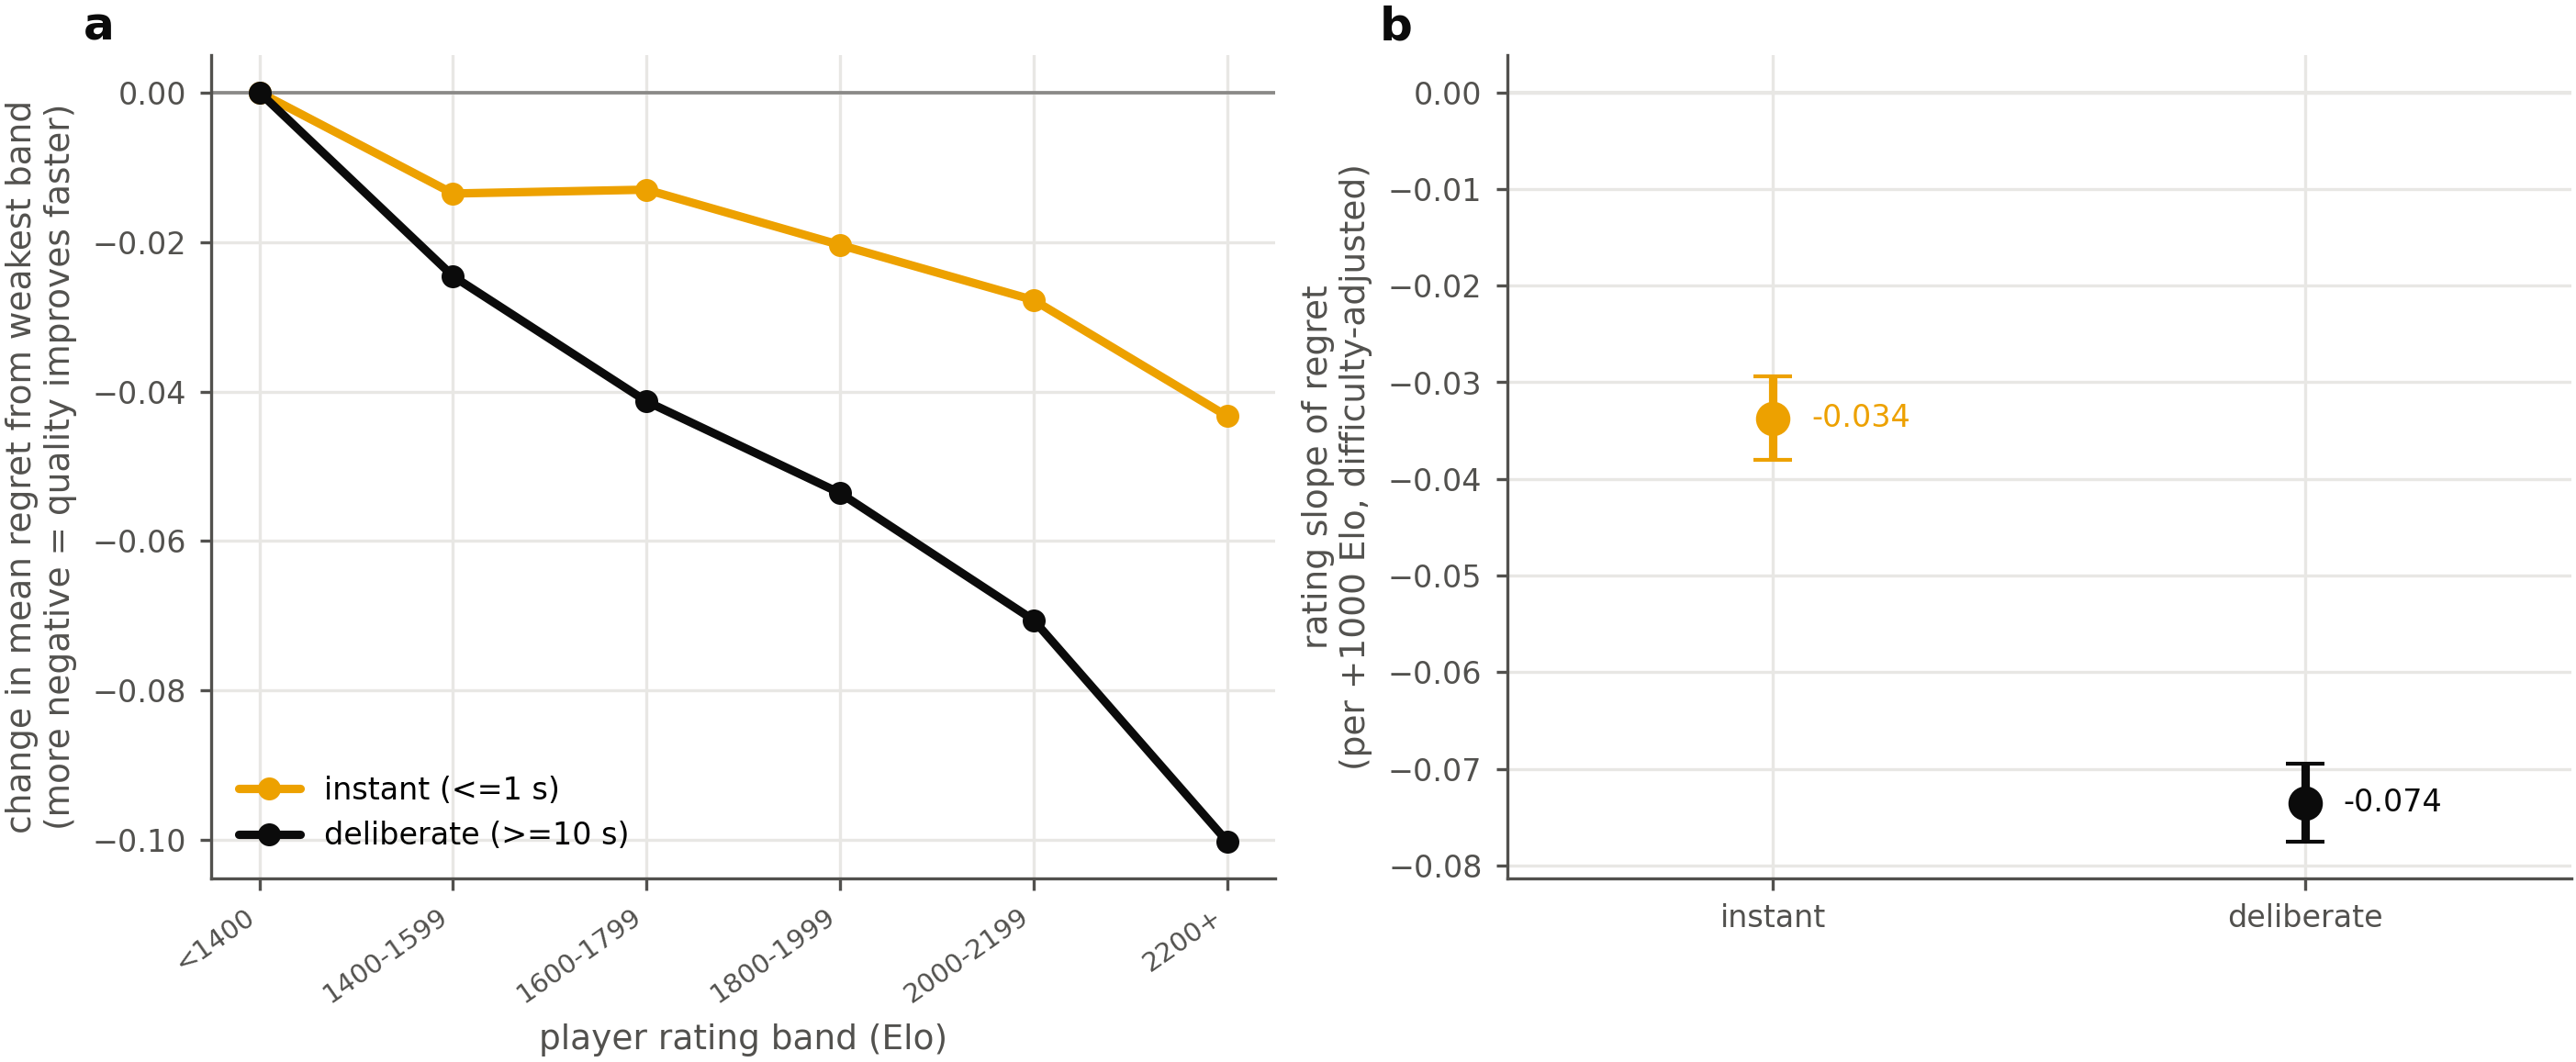
\includegraphics[width=0.92\linewidth]{figs/figR_instant_moves.png}
\caption{\textbf{Deliberation amplifies the skill gap.} Moves played instantly (${\le}1$\,s,
amber) versus deliberated (${\ge}10$\,s, dark), in non-forced positions with a healthy clock.
To avoid the recognition-based selection that makes raw quality levels non-comparable between
the groups (instant moves are self-selected as easier), the figure shows only the rating
gradient \emph{within} each group. \textbf{a}, Change in mean played-move regret relative to
the weakest rating band (each group anchored at its own baseline); the deliberated curve
descends about twice as steeply, so quality improves faster with rating when players have time
to search. \textbf{b}, Difficulty-adjusted, player-clustered slope of regret on rating
(per $1000$ Elo) for each group, with $95\%$ confidence intervals; the two do not overlap. The
pattern replicates in all four data pools (instant $-0.029$ to $-0.034$; deliberated $-0.072$
to $-0.079$).}
\label{fig:instant}\end{figure}
